\ac{General comments: the paging of the figuers is all messed up, but I will fix
it once we know what we want to keep (and discard).} 

The NTK, introduced in Sec.~\ref{sec:GradFlow}, provides a powerful framework for understanding neural
network dynamics during training. Originally developed by Jacot et
al.~\cite{jacot2018neural} to analyse infinite-width feed-forward networks, the
NTK theory has since been extended to diverse architectures including
convolutional networks~\cite{arora2019exact} and recurrent
networks~\cite{alemohammad2021recurrent}. This theoretical framework has proven
invaluable for characterizing learning dynamics and generalization properties
across various network designs.

From Eqa.~\eqref{eq:NTKDef} and~\eqref{eq:FlowEquationNoIndices}, we observe that the NTK encodes the
dependence on the architecture of the network and governs its training dynamics.
The analysis of the NTK properties is thus crucial for understanding the 
behaviour of the network during training. We first discuss the properties of the NTK at
initialisation, before moving to the training phase, where we provide a detailed
study of the NTK in the context of the NNPDF methodology. To this end, we
performed a fit of $T_3$ using the NNPDF methodology with the dataset described
in Sec.~\ref{sec:DataSet}. We initialized an ensemble of $N_{\rm Rep} = 100$ replicas with
identical architecture, training each replica independently using gradient
descent (GD) optimization. As our focus here is on NTK properties rather than
physical predictions, we use synthetic data with controlled noise
characteristics, namely L0, L1, and L2 data generations. Throughout the training process, 
we track the evolution of the NTK to understand how the network's effective
dynamics change as it learns the target function.

\subsection{NTK at Initialization}
\label{sec:NTKAtInit}
We first discuss the properties of the NTK at initialisation, that is when the
network is blind to data. We remind that, at this stage, the NTK depends on the
$x$-grid of input and on the architecture. It is argued in the literature that,
in the large-width limit, the variance of the NTK over the set of replicas tends to zero 
with the width of the hidden layers (see, \textit{e.g.}, \cite{Roberts:2021fes}). In order to
quantify the variation of the NTK, we start by computing the Frobenius norm of the NTK over
an ensemble of networks for different architectures. For each architecture, we
consider the mean value and standard deviation of the norm as statistical estimators of the
variations of the NTK. The result is displayed in Fig.~\ref{fig:NTKInit}. Even though the 
Frobenius norm is a coaarse indicator of the variations of the NTk,
the figure shows clearly that the variance of the norm becomes smaller with the size of the
network, which is consistent with the theoretical expectation that the NTK should not 
fluctuate for infinite-width networks. Note that, in addition to the scaling $\mathcal{O}(1/n)$ theoretically
predicted for large networks, the uncertainty bands include bootstrap errors
due to the finite size of the ensemble. \ac{I can say something more here.}
\ldd{Yes, you need to be more quantitative}

% ===================================
\begin{figure}[ht!]
  \centering
  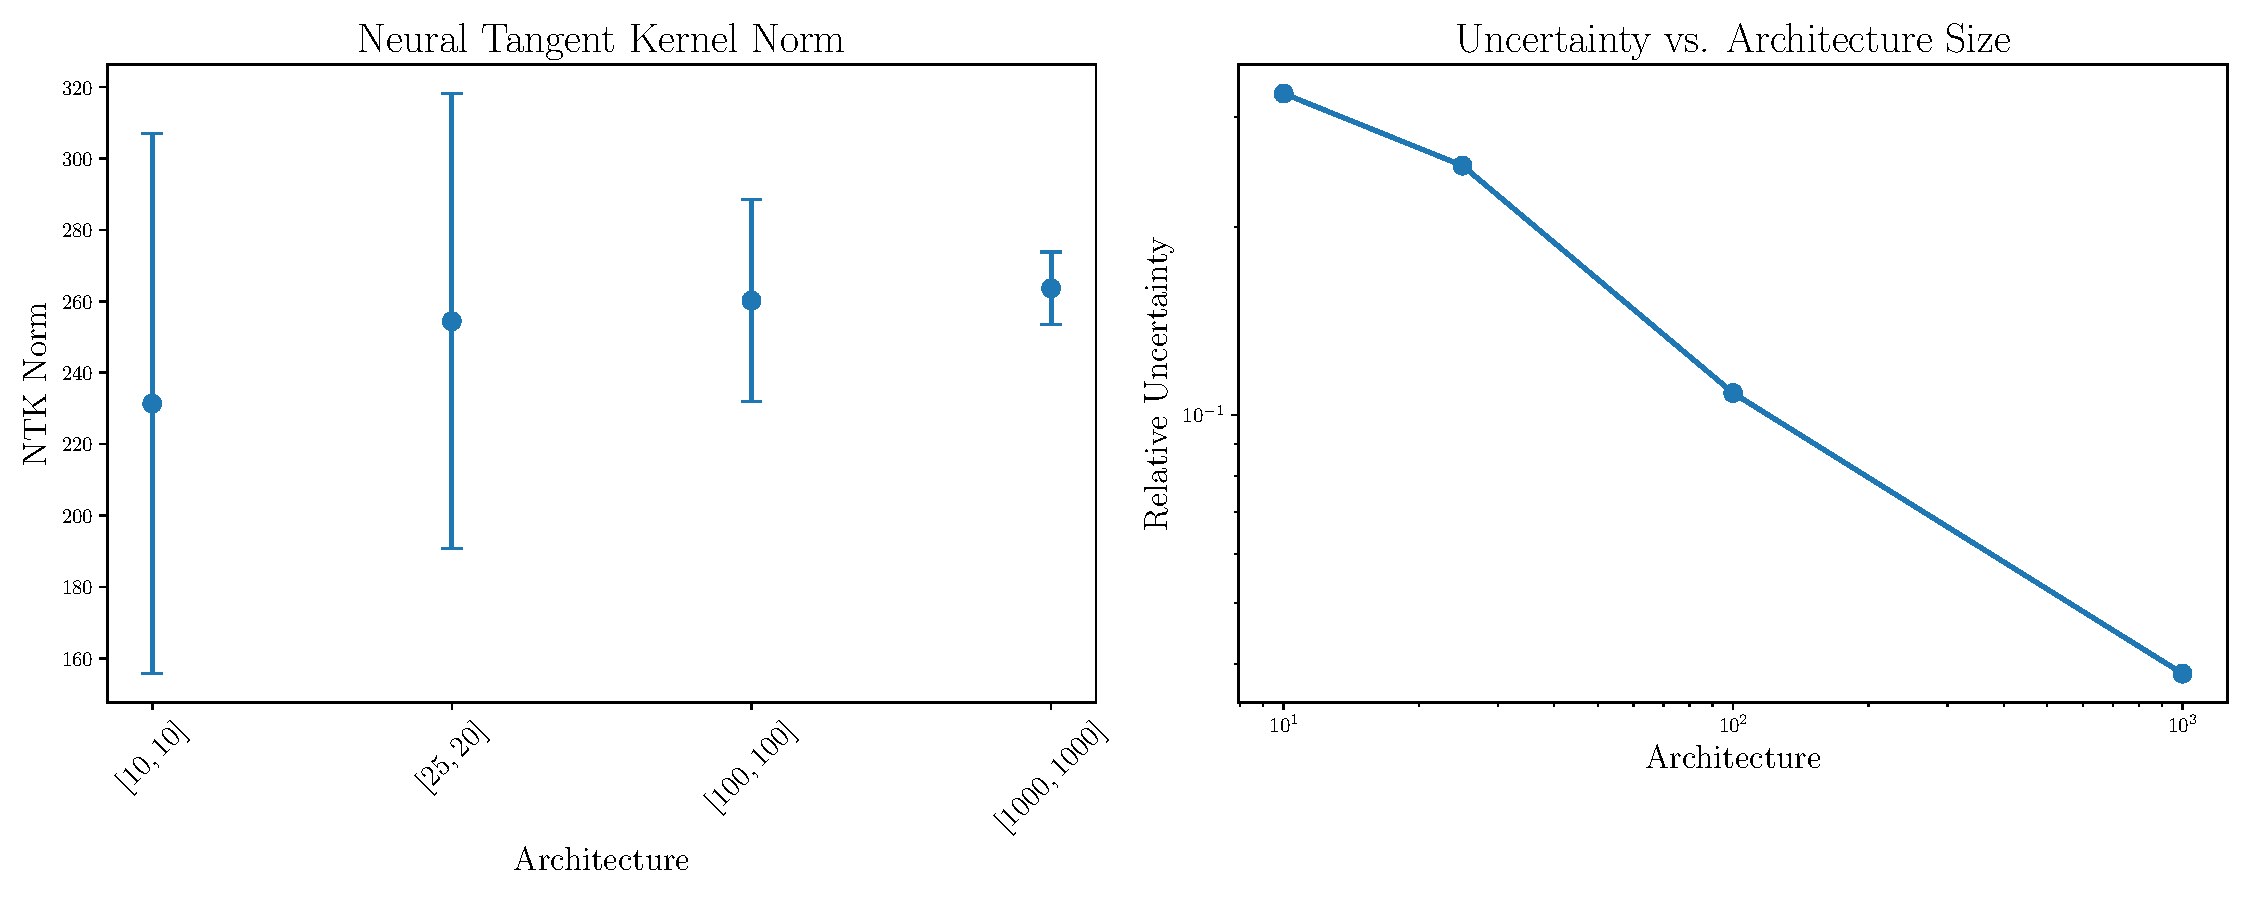
\includegraphics[width=0.90\textwidth]{../plots/ntk_pheno/ntk_initialization_with_uncertainty.pdf}
  \caption{Frobenius norm of the NTK at initialisation, $\lVert \Theta_0
  \rVert$, in function of the width of the network. On the left, the central values
  and uncertainty bands are obtained as the mean and one-sigma deviation of the
  ensemble of networks. The plot on the right shows the relative uncertainty }
  \label{fig:NTKInit}
\end{figure}
% ===================================

In order to get a more quantitative understanding of the fluctuations 
at initialization, the spectrum of the NTK is shown in Fig.~\ref{fig:NTKSpectrum} for four different architectures. 
As debated in the
literature, the spectrum of the NTK is heavily hierarchical, and only few
eigenvalues are actually non-zero\footnote{Note that, due to the large
difference in magnitude of the eigenvalues, the finite precision used in our
codes introduces noise in the decomposition, so that small eigenvalues
should be effectively considered zero. We discuss the cut-off tolerance
later, when we discuss the training process in more details.}. This means that
only a small subset of active directions can inform the network during training,
as it will be discussed later. Note that, at least at initialization, these
observations do not depend on the architecture. The eigenvalues in Fig.~\ref{fig:NTKSpectrum} 
are mostly independent of the size of the network. There is a downward fluctuation of the third
eigenvalue for the largest architecture that we considered, but we do not have any 
evidence that this drop is a physical feature of the system, rather than a fluctuation. 
the variance of the set of eigenvalues over replicas decreases with increasing 
size, as expected. 

% ===================================
\begin{figure}[ht!]
  \centering

  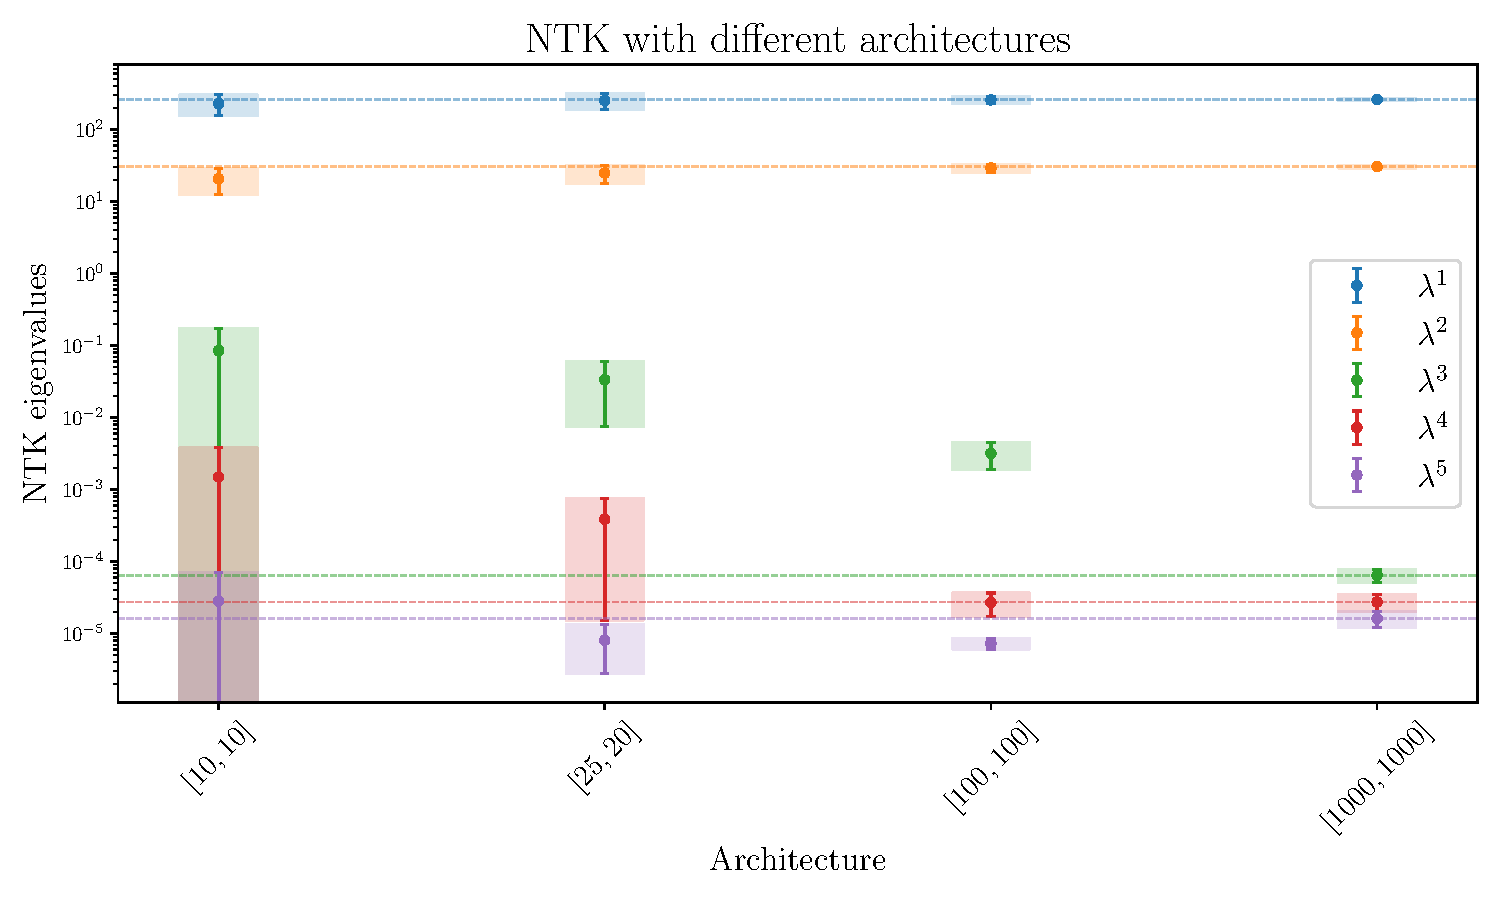
\includegraphics[width=0.90\textwidth]{../plots/ntk_pheno/ntk_initialization_arch.pdf}
  \caption{Spectrum of the NTK at initialization for the architectures shown in
  Fig.~\ref{fig:NTKInit}. }
  \label{fig:NTKSpectrum}
\end{figure}
% ===================================

\subsection{NTK During Training}
Having established the properties of the NTK at initialisation, we now discuss
its behaviour during training. In the machine learning literature, it is argued
that the NTK remains constant during training provided that the width of the
network is large enough. Here we show that this is not the case, at least for
the architectures used in the standard NNPDF methodology. 

\paragraph{Onset of lazy training.} As a first estimator of the variation of the
NTK, we show in Fig.~\ref{fig:NTKTime} the 
Frobenius norm of the variation
during training, normalized by the Frobenius norm of the NTK itself, 
\begin{equation}
\delta \Theta_t = \frac{\lVert \Theta_{t+1} - \Theta_t \rVert}{\lVert \Theta_t \rVert} \;,
\label{eq:DeltaNTK}
\end{equation}
for three different datasets, L0, L1, and L2. 

% ===================================
\begin{figure}[ht!]
  \centering
  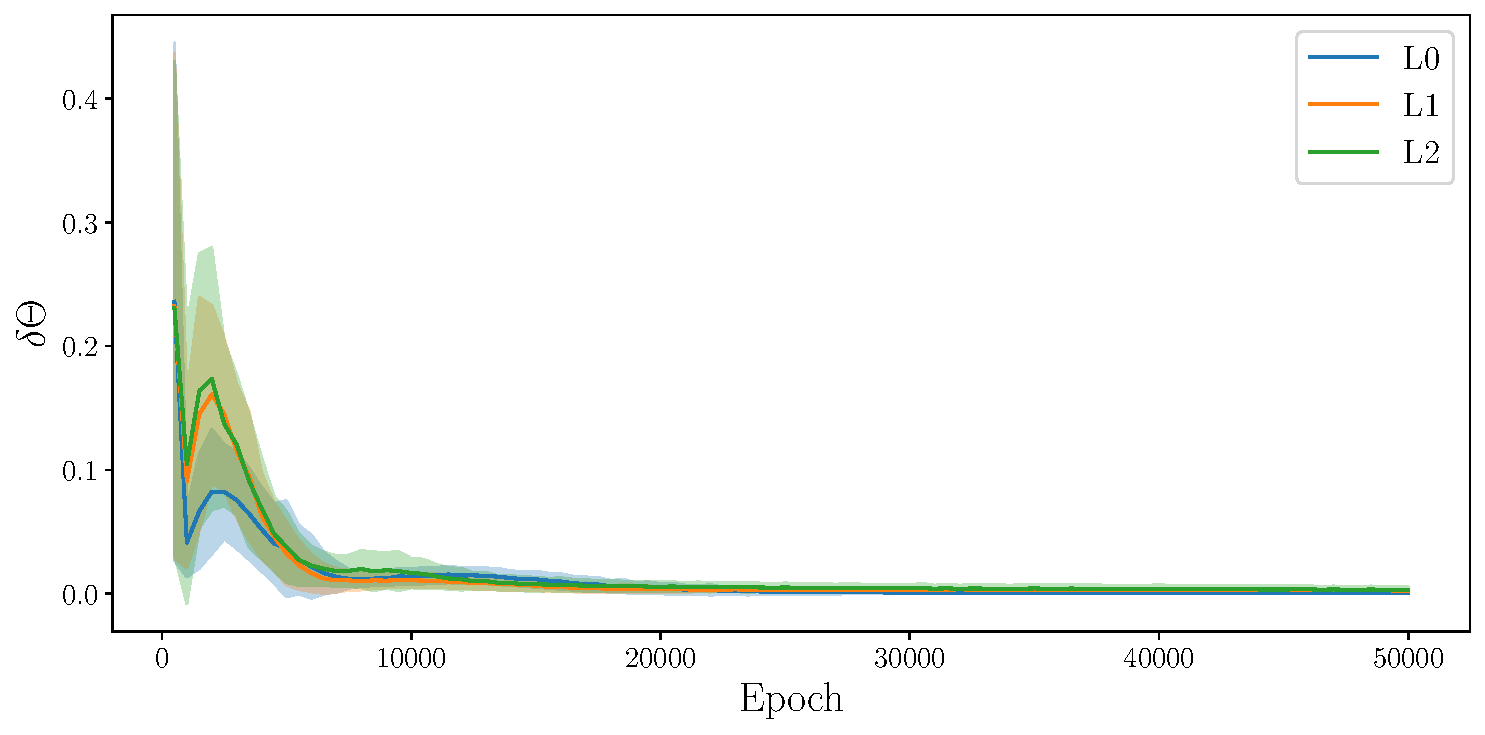
\includegraphics[width=0.6\textwidth]{../plots/ntk_pheno/delta_ntk.pdf}
  \caption{Relative variation of the NTK during training for L0, L1, and L2
  data. Error bands correspond to one-sigma uncertainties over the ensemble of
  networks.}
  \label{fig:NTKTime}
\end{figure}
% ===================================

It is clear from our data that the NTK does not remain constant during training. 
Two different phases can be distinguished in the figure. The first one
covers the initial part of the training. From Fig.~\ref{fig:NTKTime}, we see
that the norm of the NTK varies significantly in the early stages of the evolution, in strong contrast with 
the predictions obtained in the infinite-width limit. Note also that this
initial peak is more pronounced for L2 data. This is consistent with the fact
that the NTK (\ie\ the architecture) needs to accommodate the noise in
the data, thus leading to a larger variation of the NTK. On the other hand,
after this initial phase -- corresponding approximately to the first 20,000 epochs in our experiment --
the NTK tends to stabilize. As discussed in the previous Section, we refer to this
second phase as the \textit{lazy training}, in keeping with the terminology
adopted in the literature. We conclude that, in this phase, the NTK does not
change significantly. As a consequence, this suggests that a description of 
the training using a constant NTK, as predicted by the theory of the
infinite-width networks, can only be applied after the initial
phase, \ie\ after the NTK has stabilized. 

\FloatBarrier

\paragraph{Eigensystem of the NTK.}
Further insight on the evolution of the NTK can be obtained by studying its eigensystem as 
a function of the training time. 
In Fig.~\ref{fig:EigvalL0Training} we report the variation of the first five eigenvalues 
of the NTK, using the standard NNPDF architecture and L0 data. We see that the hierachical
structure observed at initialization is preserved, but the size of the subdominant eigenvalues
increases significantly in the early stages of training -- by one or two orders of magnitude depending on the 
specific eigenvalues. 
% ===================================
\begin{figure}[ht!]
  \centering  
  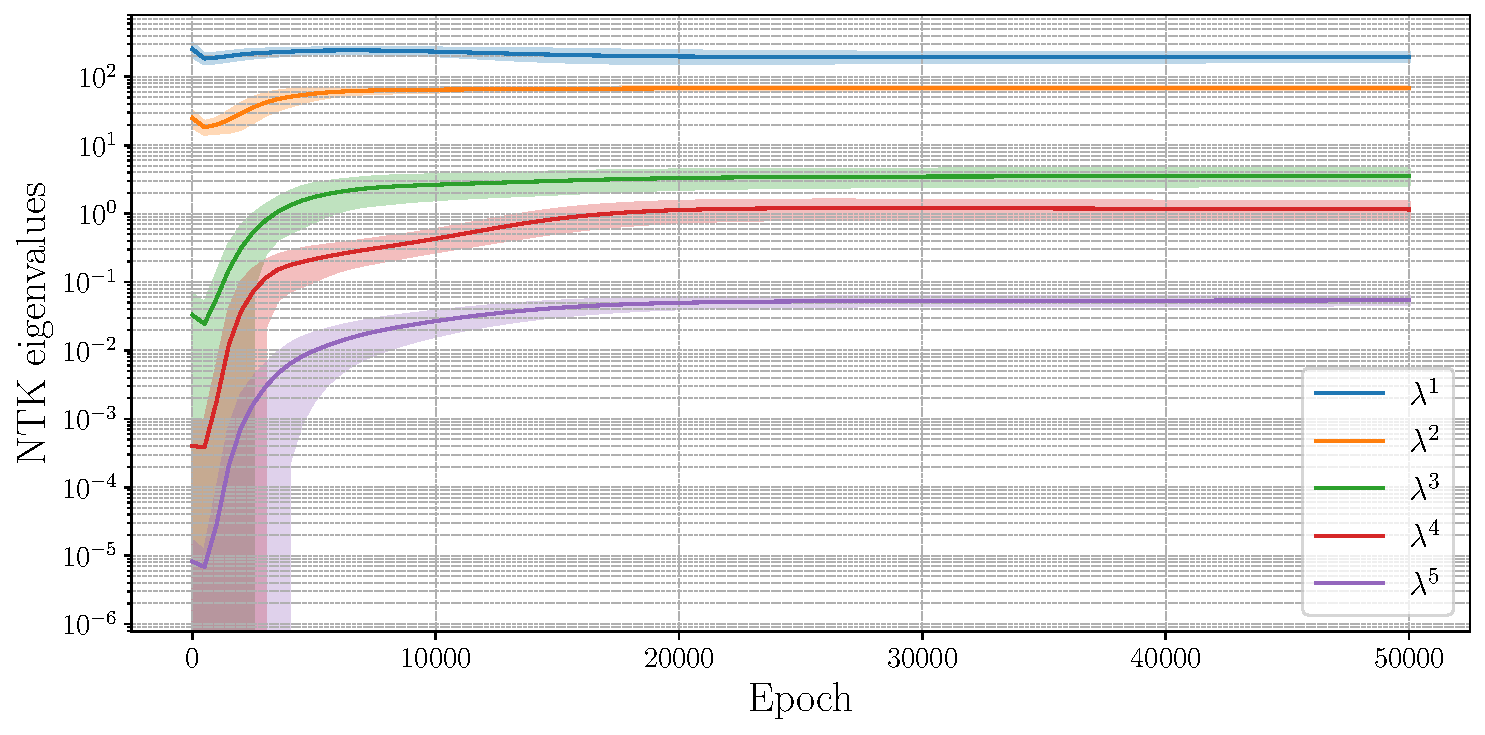
\includegraphics[width=0.78\textwidth]{plots/ntk_pheno/ntk_eigvals_single_plot_L0.pdf}  
  \caption{Evolution during training of the first five eigenvalues of the NTK.}
  \label{fig:EigvalL0Training}
\end{figure}
% ===================================
In Fig.~\ref{fig:EigvalsComparison}, the same first five eigenvalues of the NTK
are displayed for L0, L1, and L2 data. We can make a few observations upon
inspecting these plots. First, we notice that the way in which data is generated
has an impact on the eigenvalues of the NTK. In general, the uncertainty bands
for L2 data are larger than those for L1 and L0 data, indicating that the NTK is
more sensitive to the noise in the data. This is consistent with the observation
made in Fig.~\ref{fig:NTKTime}. 
The eigenvalues reach a plateau and do not change significantly once 
the network enters the lazy training regime. This fact, combined with the analysis of Eq.~\eqref{eq:FlowSolution}, 
suggests that more ``physical'' features become learnable before lazy training sets in. 

% ===================================
\begin{figure}[ht!]
  \centering
  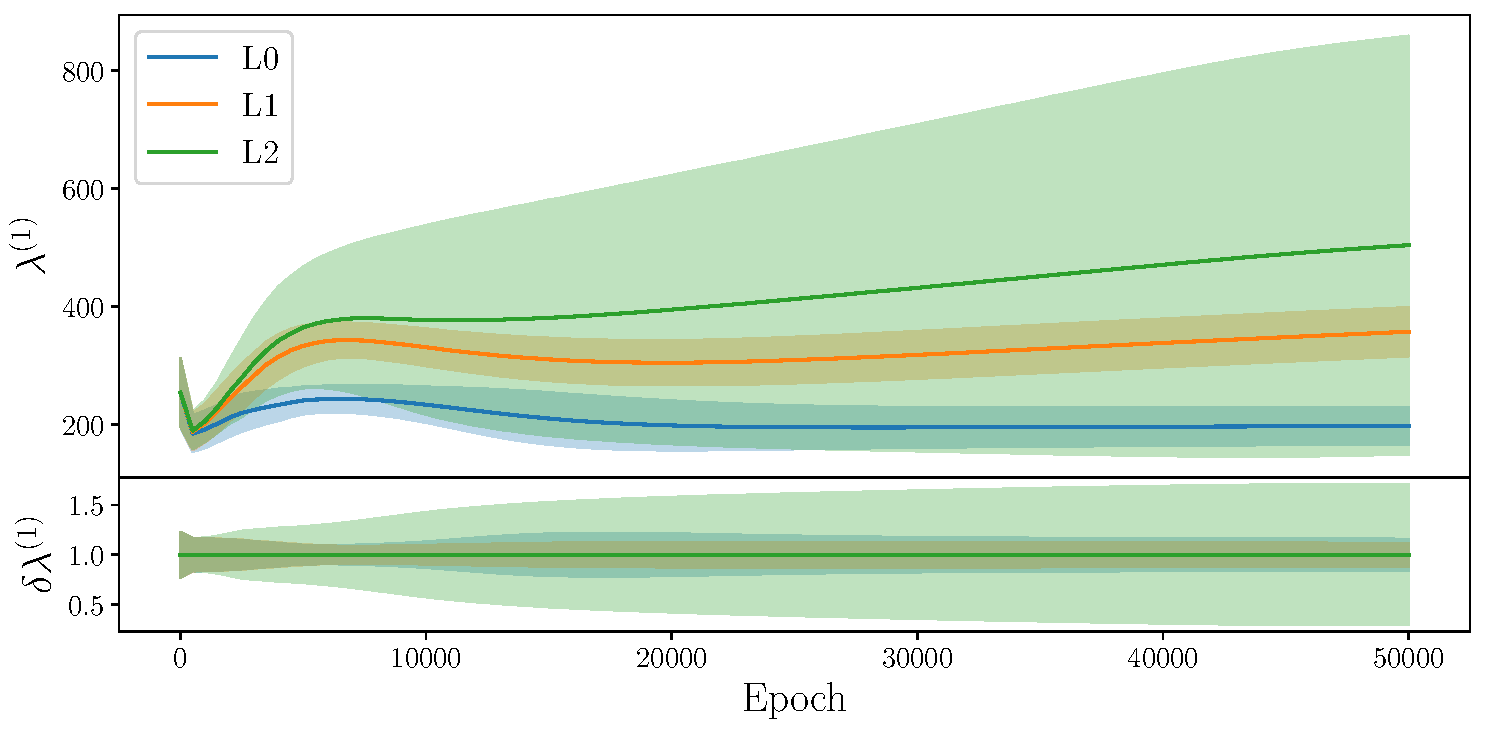
\includegraphics[width=0.48\textwidth]{../plots/ntk_pheno/ntk_eigvals_L0_L1_L2_n_1.pdf}
  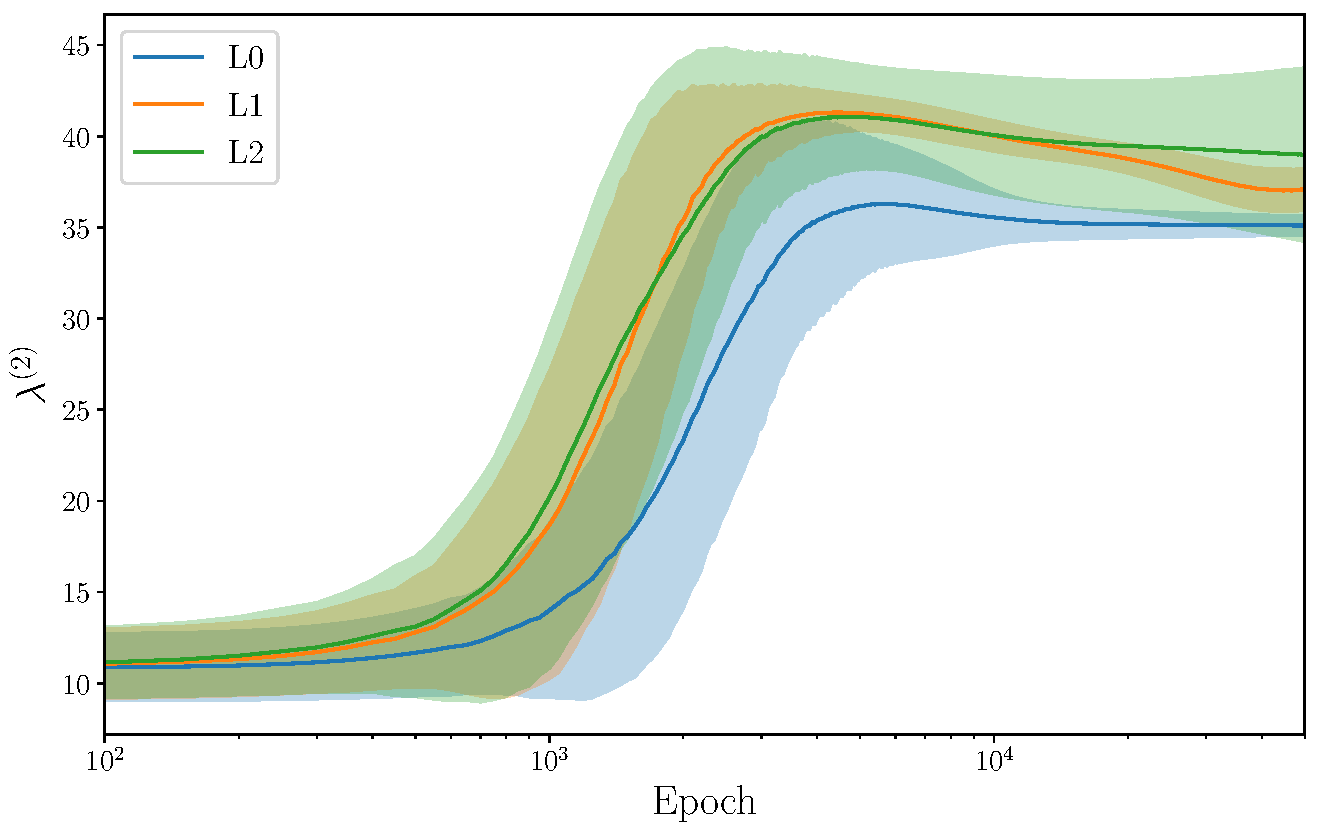
\includegraphics[width=0.48\textwidth]{../plots/ntk_pheno/ntk_eigvals_L0_L1_L2_n_2.pdf}
  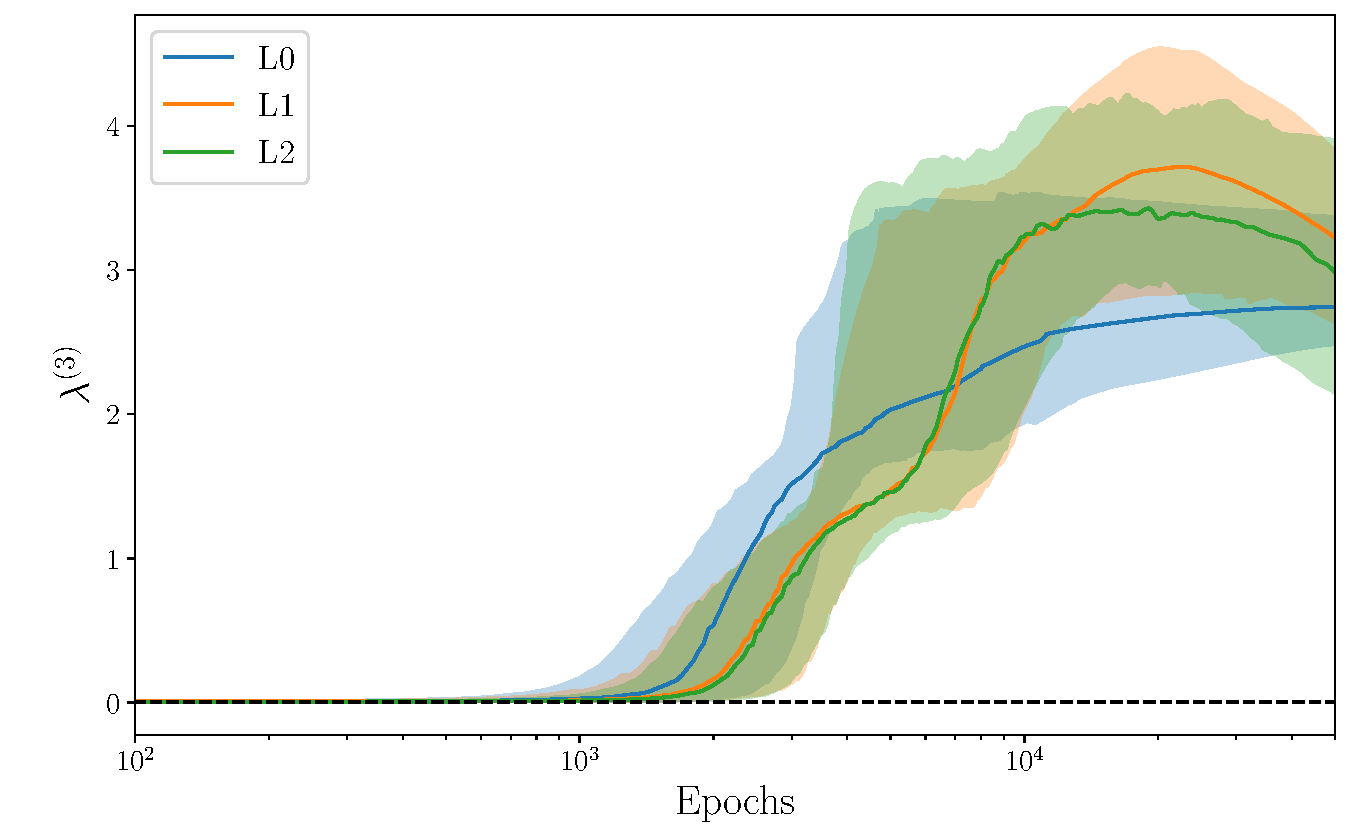
\includegraphics[width=0.48\textwidth]{../plots/ntk_pheno/ntk_eigvals_L0_L1_L2_n_3.pdf}
  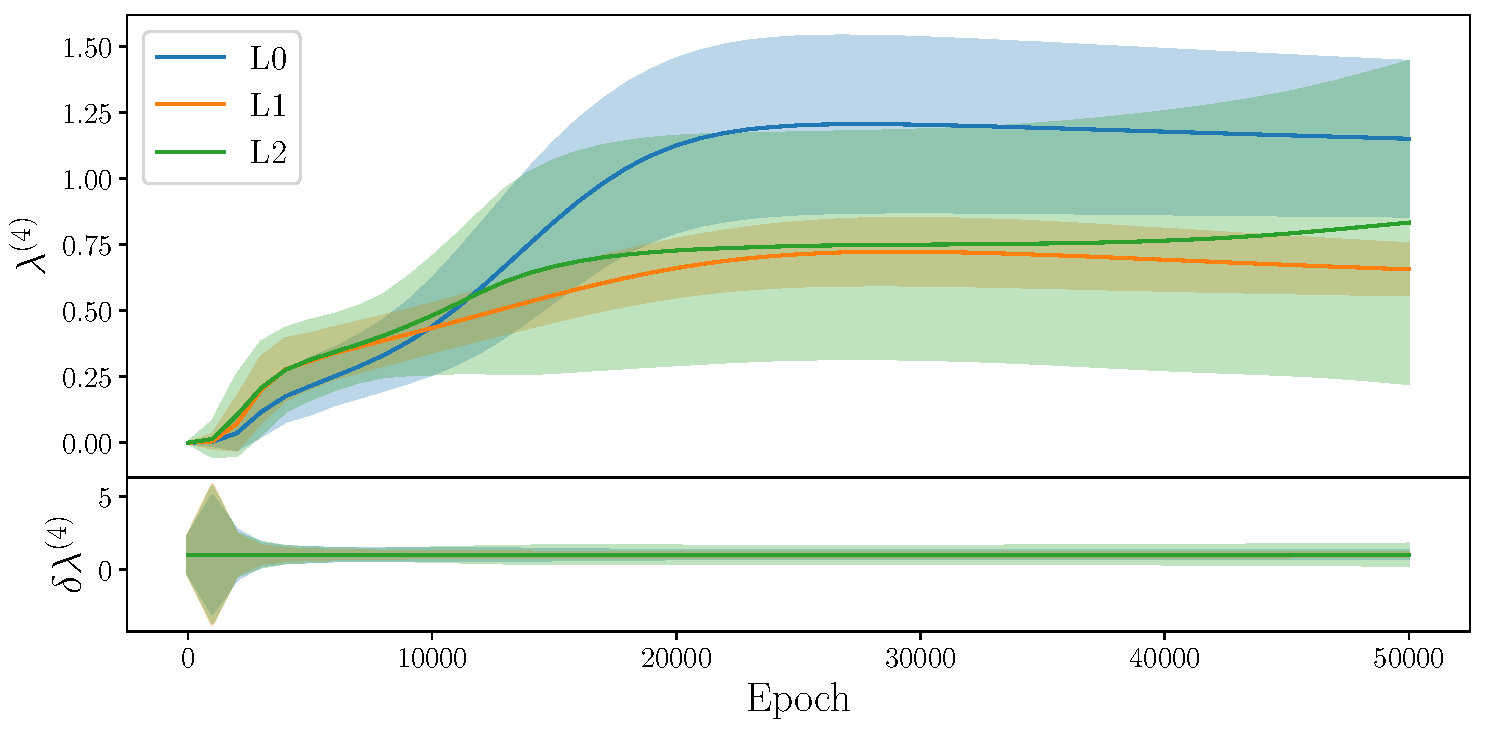
\includegraphics[width=0.48\textwidth]{../plots/ntk_pheno/ntk_eigvals_L0_L1_L2_n_4.pdf}
  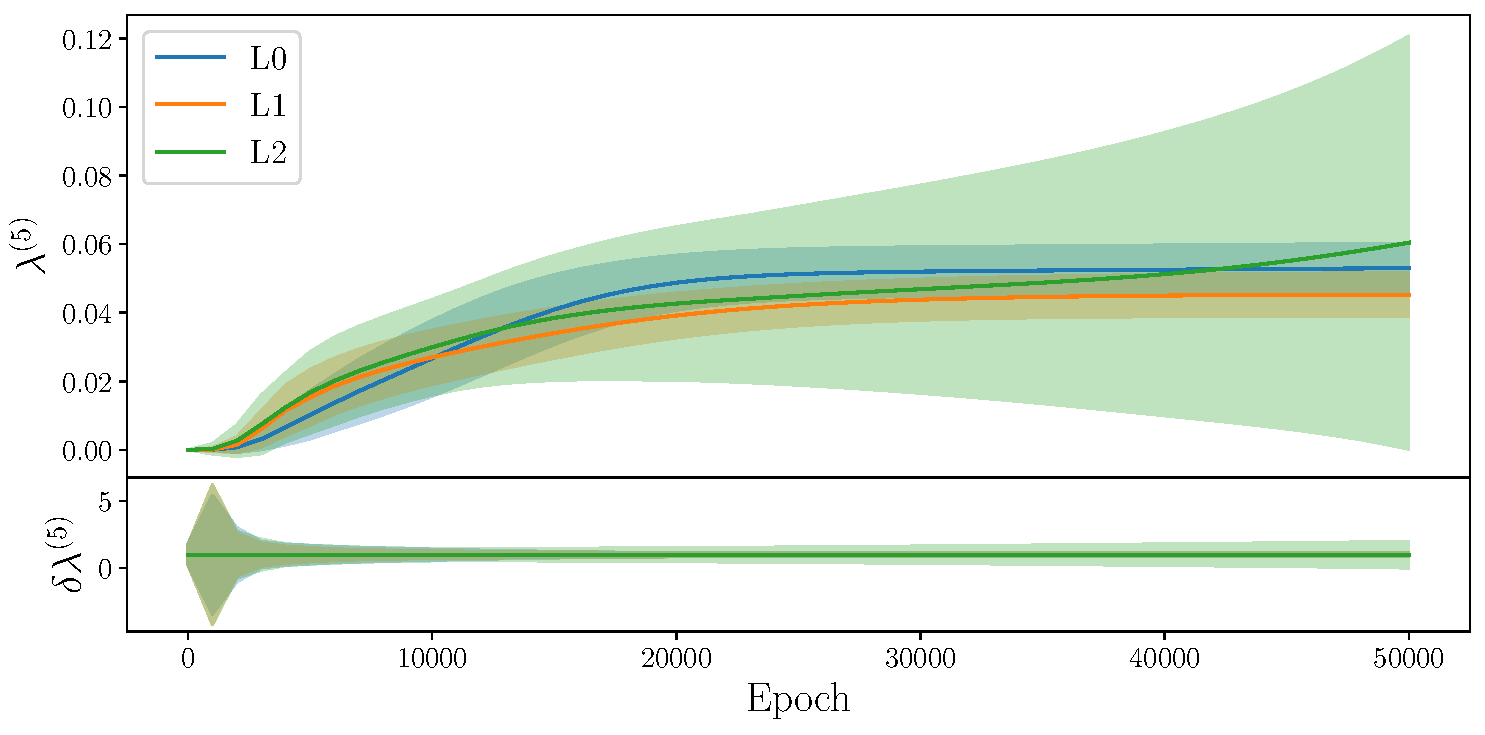
\includegraphics[width=0.48\textwidth]{../plots/ntk_pheno/ntk_eigvals_L0_L1_L2_n_5.pdf}
  \vspace{0.5cm}
  \caption{The first five eigenvalues of the NTK for L0, L1, and L2 data. Error
  bands correspond to one-sigma uncertainties over the ensemble of networks.}
  \label{fig:EigvalsComparison}
\end{figure}
% ===================================

\FloatBarrier

\paragraph{Dependence on the architecture.}
In order to learn more about the onset of lazy training, it is interesting to consider what happens to 
the picture sketched so far as the architecture of the neural networks is varied. In Fig.~\ref{fig:NTKTimeDiffArch}
we compare the time dependence of the Frobenius norm of the NTK and the variation of the first three eigenvalues
for two different architectures. The smaller network is the $[28,20]$ used in the standard NNPDF
analyses and in this work, while the large one is a $[100,100]$ network, which is closer to the infinite-width
limit. For illustration purposes we focus in this plot on L1 data and only three eigenvalues rather than the five
we examined above. The quantitative features are exactly the same for L0 and L2 data, and adding the fourth 
and fifth eigenvalues does not add unexpected behaviours compared to what we observe in Figs.~\ref{fig:NTKTime} 
and~\ref{fig:EigvalL0Training}. It is interesting to remark that the onset of lazy training is slower 
for the larger network. This is to be expected if we interpret the onset of lazy training as a phase where 
the network identifies the learnable features in the space of functions that it can parametrize. For a 
larger network, the space of parametrized functions is larger and the identification of the physical 
features takes a larger number of epochs. 
% ===================================
\begin{figure}[ht!]
  \centering
  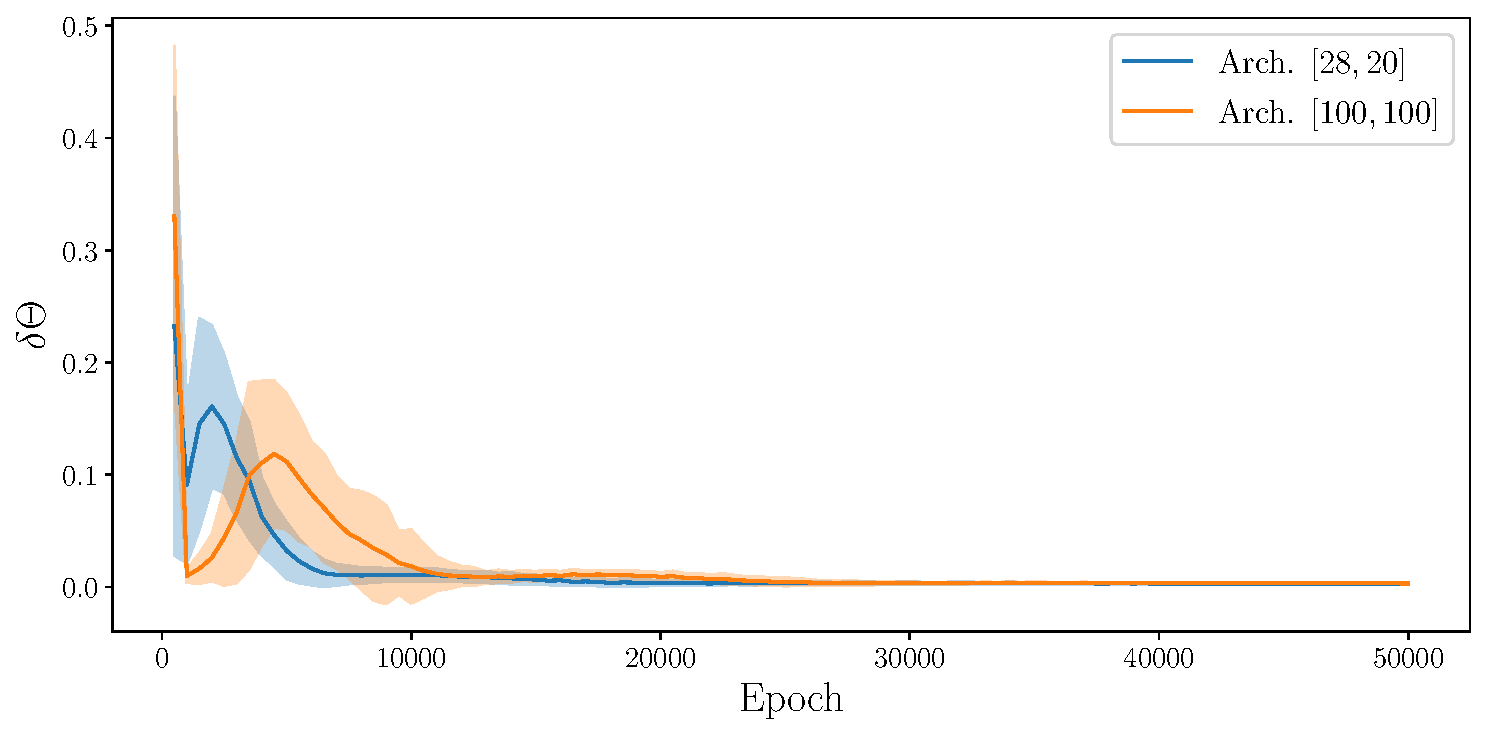
\includegraphics[width=0.45\textwidth]{../plots/ntk_pheno/delta_ntk_arch.pdf}
  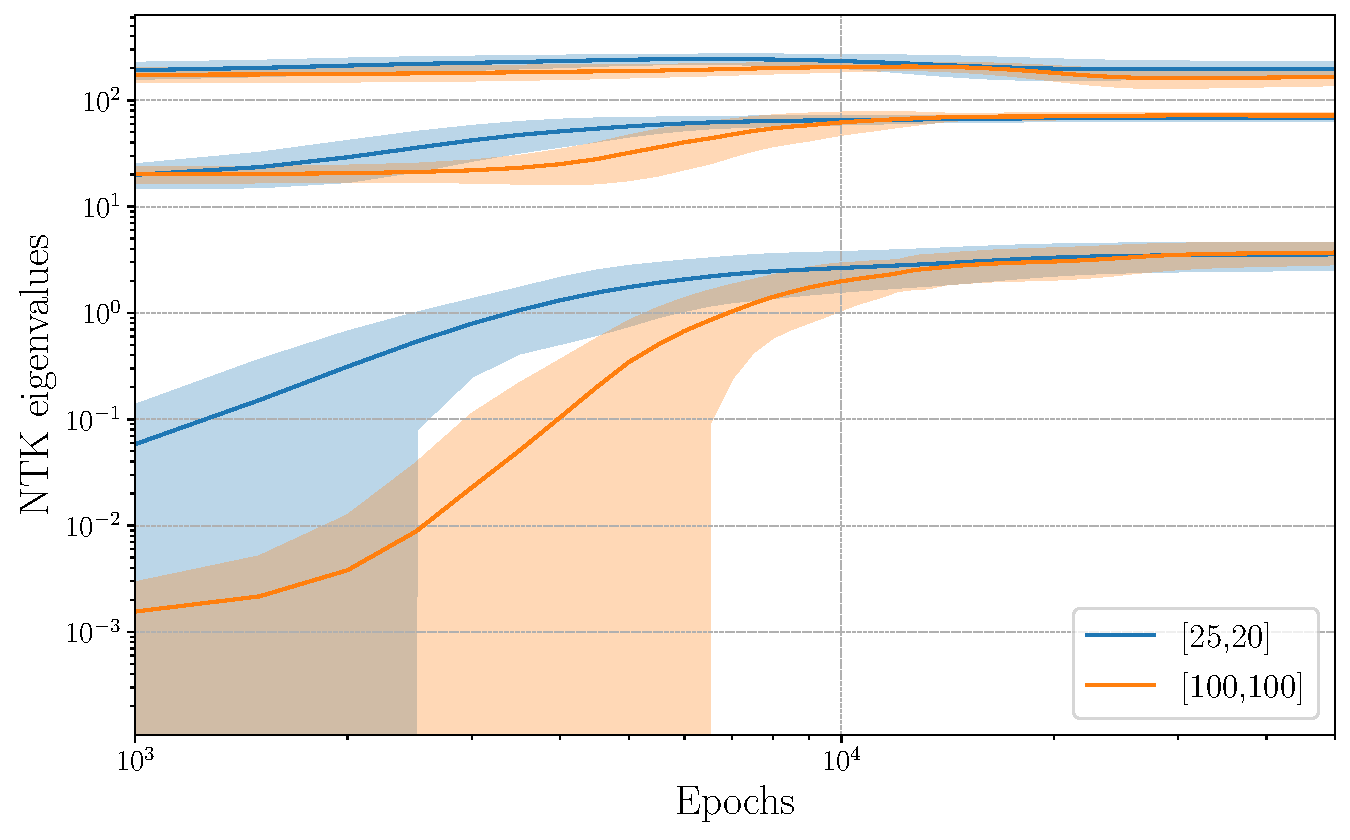
\includegraphics[width=0.45\textwidth]{../plots/ntk_pheno/ntk_eigvals_single_plot_arch.pdf}
  \caption{Comparison of the variation of the NTK during training (left) and the
  first three eigenvalues (right) for two different architectures with sizes
  $[28,20]$ and $[100,100]$ respectively. In both cases, L1 data is used. Error
  bands correspond to one-sigma uncertainties over the ensemble of networks.}
  \label{fig:NTKTimeDiffArch}
\end{figure}
% ===================================

\FloatBarrier

\paragraph{Alignment of the NTK.}
It has been argued before that there is a non-trivial interplay between the
eigenspace of the NTK and that of the matrix $M$. Indeed, the former encodes the
model dependence, while the latter brings physical information. Of course the
two matrices are independent at initialisation, and we do not expect any
alignment patter between the two. However, this picture does change during
training, as the NTK evolves and the model learns the target function. To
quantify this alignment, we define the matrix $A$, 
\begin{equation}
  \label{eq:MatrixA}
  A_{kk'} = \left( \left< z^{(k)}, v^{(k')}\right> \right)^2 = \cos^2(\theta_{kk'}) \;,
\end{equation}
where $z^{(k)}$ and $v^{(k')}$ are the $k$-th and $k'$-th eigenvectors of the
NTK and $M$, respectively. The matrix $A$ is thus a measure of the alignment
between the eigenspaces of the two matrices. The rows of the matrix correspond to 
the eigenvectors of the NTK, ordered by the value of the corresponding eigenvalues, 
with the eigenvectors corresponding to the larger 
eigenvalues at the top of the matrix. The columns correspond to eigenvectors 
of the matrix $M$, also ordered by the values of the corresponding eigenvalues, 
with the largest eigenvalues to the left in this case. In Fig.~\ref{fig:NtkMAlign}, we
show the matrix $A$ at different epochs of the training for L2 data and a
single NTK replica. 
% ===================================
\begin{figure}[ht!]
  \centering
  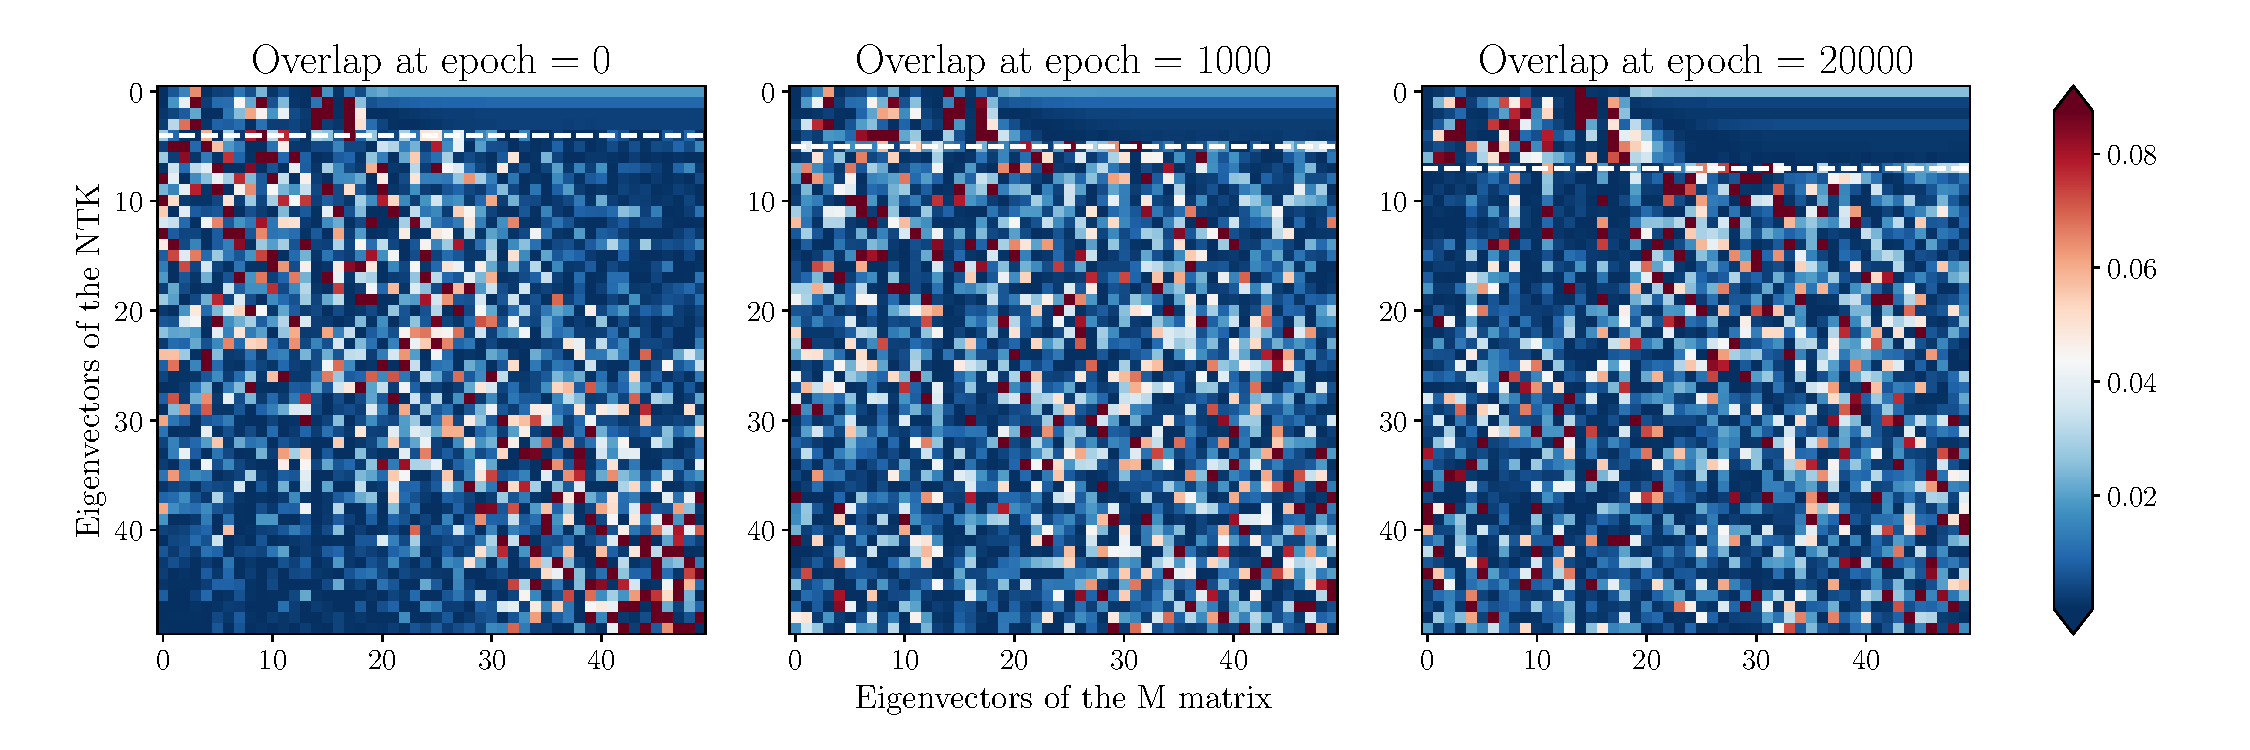
\includegraphics[width=1\textwidth]{plots/ntk_pheno/ntk_alignment.pdf}
  \caption{Matrix $A$ as defined in Eq.~\eqref{eq:MatrixA} for L1 data and for a
  single replica of the NTK. The matrix is shown at different epochs of the
  training process, indicated in the top of each panel. The white dashed line
  indicates the cut-off tolerance that we imposed to the eigenvalues of the NTK
  (see Appendix...?).}
  \label{fig:NtkMAlign}
\end{figure}
% ===================================
The blue rectangle in the top right corner of the matrix shows that the eigenvectors
of the NTK corresponding to the largest eigenvalues are orthogonal to the eigenvectors
of $M$ that are in the kernel of $M$, \ie\ the directions that do not contribute to the 
observables. It is useful to remember that the largest eigenvalues of the NTK correspond 
to the directions that are orthogonal to $\ker\Theta$, \ie\ the directions that are learnable
during the training process. In order to have a robust training process, we expect these 
learnable directions to align with the directions that actually contribute to the loss 
functions, \ie\ the ones corresponding to the largest eigenvalues of $M$. Consistently with 
this intuition, we see that the size of this blue rectangle increases with training time. 
In particular, it is clear from our plot that it becomes deeper by the onset of the lazy 
training regime: more of the learnable directions -- the {\it features}\ that the network 
can learn -- are aligned with the directions that contribute most to the observables. 

\FloatBarrier
